\documentclass[portrait, a0]{a0poster}
%\documentclass[landscape, a0]{a0poster}

\pagestyle{empty}
\setcounter{secnumdepth}{0}

\usepackage[absolute]{textpos}
\usepackage{graphicx}
%\usepackage{charter}
\usepackage{palatino}
\usepackage{mflogo}
\usepackage{url}

\usepackage{caption}
\captionsetup{font=small, labelfont={sf,bf}, textfont=it}

\usepackage{color}
\definecolor{DarkBlue}{rgb}{0.1,0.1,0.4}

\TPGrid[40mm,40mm]{26}{12}      % 3 cols of width 8, plus 2 gaps width 1

\parindent=0pt
\parskip=0.5\baselineskip

\def\Heading#1{\noindent{\hfill{\LARGE{\color{DarkBlue} \bf #1}}}\medskip\hrule}
\def\SHeading#1{\medskip\par\noindent{\Large\color{DarkBlue} \it #1}\medskip}
\def\SSHeading#1{\medskip\par\noindent{\large\color{DarkBlue} #1}\medskip}

\begin{document}

%include heading
\begin{textblock}{26}(0,0)
    \centering
    \VeryHuge{Particle Swarm Frequency Planning}
\end{textblock}

%include names
\begin{textblock}{26}(0,1)
 \begin{center}
   \Large{W. Bezudienhout, G.B O'Reilly} \\
   \Large{Academy for Information Technology} \\
   \Large{University of Johannesburg} \\
 \end{center}
\end{textblock}

%include logo
\begin{textblock}{8}(18,11)
\centering

\includegraphics{pics/ujlogo.pdf}
\end{textblock}

%col 1
\begin{textblock}{8}(0,2)
\Heading{Steganographic File Systems}

\SHeading{Traditional Steganography}

Traditional steganography, or \emph{information hiding}, is an extension to the field of information security. Traditional steganographic techniques aim to embedded data within an unassuming ``cover--object''.

Image and audio steganography are the most well--known of these techniques, where hidden data is embedded within an image or audio file. These techniques have limitations, as the maximum amount of information which can be embedded is determined by the overall \emph{``dimensions''} of the cover--object.

\SHeading{What is a Steganographic File System?}

Steganographic file systems allow relatively large amounts of data to be securely embedded within a \emph{``cover file system''}. Hidden data is embedded along side non--hidden data (or host data), on a single physical device.

Steganographic file systems strive to manage the interaction between the hidden and non--hidden data. There are a number of existing steganographic file system implementations.

\begin{itemize}
 \item \textsl{Anderson, Needham, and Shamir} -- describe two different methods for hiding data within a file system:
	\begin{enumerate}
		\item Data is hidden within a sub-set of cover-files. The sub-set is chosen by a stego-key.
		\item A randomly initialised disk is used to hide data -- data duplication is used to maximise disk usage, and avoid \emph{collisions}.
	\end{enumerate}
 \item \textsl{McDonald and Kuhn} -- propose an implementation that uses a modified Ext2 file system to hide data. Data must again be duplication to avoid collisions.
 \item \textsl{Pang, Tan, and Zhou} -- this implementation specifies a file system that allows data to be hidden. Data is hidden with the non--hidden data. The existence of hidden--files is obfuscated using \emph{dummy files}, and \emph{abandoned blocks}.
\end{itemize}

Steganographic file systems rely heavily on \emph{cryptography} to provide information security.

\SHeading{Information Security through Cryptography}

It is not enough to hide data on the physical disk, it would be a very simple operation to extract the hidden data from the unallocated physical blocks. Cryptography must therefore be used to ensure that hidden data will remain secure.

The hidden data will be encrypted using a \emph{block cipher}, which will encrypt data in discrete blocks. The \emph{Serpent} algorithm is a good example of a modern cryptographic block cipher which could be used.

\SSHeading{Block Cipher Modes}

Block cipher modes are used to control how the encryption process operates. Steganographic file systems store \emph{structured data}, thus the operation of the block cipher must be taken into account. The block cipher modes which we will discuss are \emph{Electronic Codebook (ECB)} mode and \emph{Cipher Block Chaining (CBC)} mode.

\emph{Electronic Codebook} mode operates by encrypting each block of the plaintext with the same encryption key. This presents a problem with structured data. As can be seen in figure~\ref{fig:ecb}, identical blocks of data will produce identical block of ciphertext.

To ensure that hidden data will remain secure, \emph{Cipher Block Chaining} mode is used for encryption. CBC mode encrypts each block with a encryption key which is derived from the previously encrypted block. As seen in figure~\ref{fig:ecb} This allows the ciphertext to remain completely indistinguishable from the original.

\begin{figure}
\centering
\footnotesize
\begin{tabular}{c c c}
\\

\includegraphics[width=6cm]{pics/hex.pdf} & 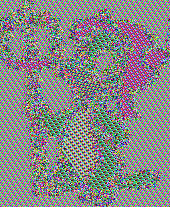
\includegraphics{pics/ecb.png} & 
\includegraphics{pics/cbc.png} \\
Original image & ECB mode & CBC mode \\
{\scriptsize \url{http://www.hexley.com}}
\end{tabular}
\caption{Comparison between ECB and CBC Block Cipher Modes \label{fig:ecb}}
\end{figure}

\end{textblock}

%col 2
\begin{textblock}{8}(9,2)
\Heading{SSFS}

The Secure Steganographic File System (SSFS) is designed to allow hidden data to be securely embedded within a host file system. SSFS strives to provide information security through information hiding techniques, and to provide a mechanism for plausible deniability.

\SHeading{Aim}

SSFS attempts to address problems with existing steganographic file system implementations. Chief among these is the management of the interaction between the hidden and non--hidden data, to ensure that no data is lost. Other design aspects of SSFS are listed below.

\begin{itemize}
\item \textsl{Security} -- hidden data must remain protected from attack through the use of effective security mechanisms. This is achieved through the use of \emph{cryptography}.

\item \textsl{Consistency} -- hidden data which is retrieved from the hidden file system must be the same as the original data which was stored. Hidden data must not be \emph{lost}.

\item \textsl{Transparency} -- operation of the host file system must not be impacted in a significant way. Hidden data must integrate transparently into the host file system.

\item \textsl{Backward Compatibility} -- SSFS must be \emph{backward compatible} with a host file system implementation. This will provide \emph{plausible deniability}.

\item \textsl{Dynamic Reallocation} -- hidden data must be able to be located from any physical location. The physical location of the hidden data must be allowed to change.
\end{itemize}

\SHeading{Construction}

SSFS is constructed as a \emph{compound file system} where the host and hidden data is managed by two distinct file system implementations. The non--hidden data is managed by the \emph{host file system}, and the hidden data is managed by the \emph{hidden file system}.

\SSHeading{Host File System}

The host file system is constructed from an existing file system, and consists of a \emph{Superblock}, a \emph{Storage Bitmap}, an \emph{Inode Bitmap}, and an \emph{Inode Table}.

For the purpose of explanation, the above structures are arranged on a physical device as seen in figure~\ref{fig:hostlayout}.

\begin{figure}
\centering
\begin{tabular}{c}
\\
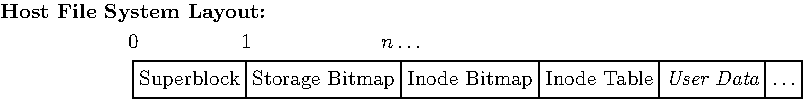
\includegraphics[scale=1.3]{pics/fig-1.pdf}
\end{tabular}
\caption{Host File System Layout \label{fig:hostlayout}}
\end{figure}

The host file system must remain \emph{backward compatible} with the original file system implementation in order to provide \emph{plausible deniability}.

\SSHeading{Hidden File System}

The hidden file system is embedded in the host file system, and provides for the management of the hidden data, and is a \emph{complete} file system implementation.

The hidden file system consists of the following structures: the \emph{Superblock}, the \emph{Translation Map}, and the \emph{Inode Table}. These structures allow the hidden data to be managed by the hidden file system implementation, and are logically positioned on the device as seen in figure~\ref{fig:hiddenlayout}.

\begin{figure}
\centering
\begin{tabular}{c}
\\
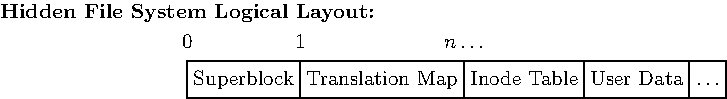
\includegraphics[scale=1.3]{pics/fig-3.pdf}
\end{tabular}
\caption{Hidden File System Layout \label{fig:hiddenlayout}}
\end{figure}

To allow for hidden data to be easily embedded in the unallocated host file system blocks, all hidden data is referenced \emph{logically} within the hidden file system implementation. The Translation Map allows hidden logical blocks to be mapped to physical locations (seen in figure~\ref{fig:logicalmappings}). This forms the basis for the \emph{dynamic reallocation} mechanism. Hidden data can exist in any physical location on the physical device, and the physical location of the hidden data need not be constant. For example, a hidden inode entry will reference associated hidden data by its hidden logical position.

\end{textblock}

%col 3
\begin{textblock}{8}(18,2)

\begin{figure}
\centering
\begin{tabular}{c}
\\
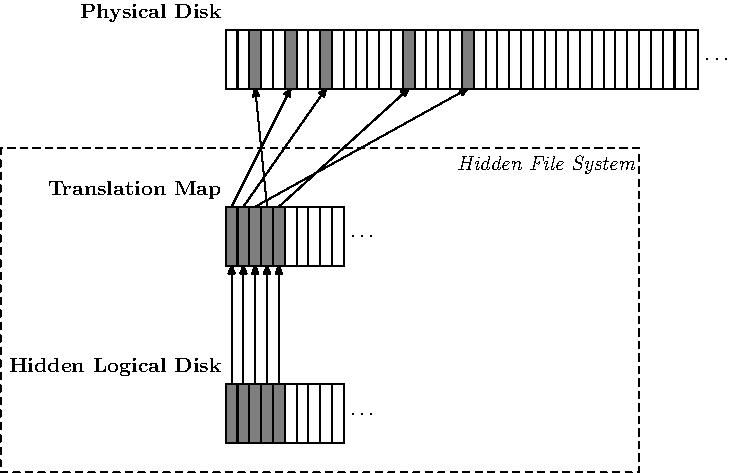
\includegraphics[scale=1.5]{pics/fig-4.pdf}
\end{tabular}
\caption{Showing the Translation Map providing the logical--to--physical mappings \label{fig:logicalmappings}}
\end{figure}

\Heading{Dynamic Reallocation}

The dynamic reallocation mechanism allows hidden data to be moved to an alternate location on the physical device, without affecting the hidden file system's control structures. Steganographic file systems suffer from collisions between the hidden and non--hidden data. The host file system will at some point request that data be written to a physical block which contains hidden data.

SSFS will dynamically reallocate hidden data to an alternate location in order to allow the host file system to safely perform the write operation. This is achievable via the Translation Map.  

The design of SSFS allows the underlying physical location of the hidden data to be changed without the need for the associated file system structures to be modified. The logical--to--physical translation mechanisms provided by the Translation Map will ensure that hidden data is always accessed correctly.

The dynamic reallocation process can be summarised in the following steps:

\begin{enumerate}
\item Intercept the host file system's \texttt{write} operation.
\item Check to see if the requested physical block contains hidden data. If it does\ldots
 \begin{enumerate}
  \item Find an alternate unallocated physical location.
  \item Move the hidden data to that physical location.
  \item Update the associated mapping in the Translation Map.
 \end{enumerate}
\item Continue with the host file system's \texttt{write} operation.
\end{enumerate}

\Heading{Results}

The effect of the \emph{dynamic reallocation} process on the host file system will determine the overall feasibility of SSFS. If the performance impact is too great, the existence of hidden data could be inferred from the extra processing overhead.

Figure~\ref{fig:graph} shows the total time taken to allocate a number of files on the host file system when the dynamic reallocation mechanism is in use. The overall processing overhead can be kept to a minimum through optimisation of the dynamic reallocation algorithm. The observed performance impact will allow such a system to be feasible.

\begin{figure}
\centering
\begin{tabular}{c}
\\
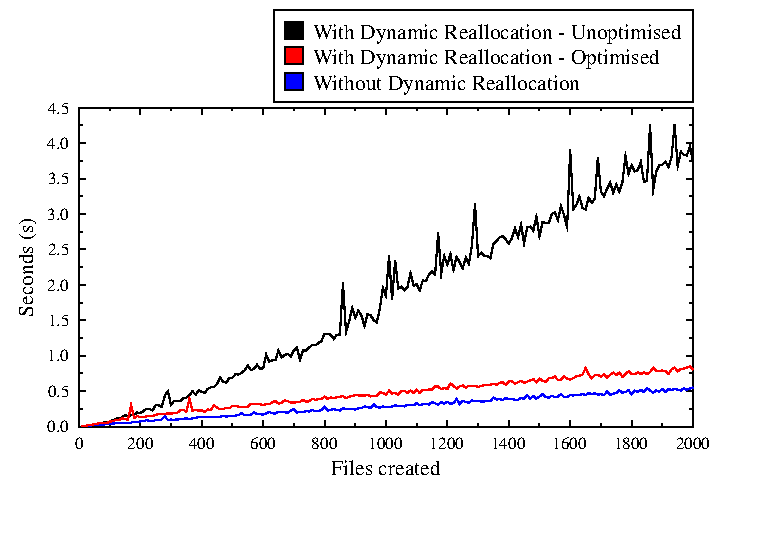
\includegraphics[scale=1.5]{pics/graph1.pdf}
\end{tabular}
\caption{Graph showing the amount of time taken to allocate a number of files in the host file system with the dynamic reallocation mechanism in operation. \label{fig:graph}}
\end{figure}

\end{textblock}

%footer
\begin{textblock}{8}(0,12)
\footnotesize
Produced using \LaTeXe\ and \MP.
\end{textblock}

\end{document}
